\firstsection{Introduction}

\maketitle

Artificial intelligence has taken the world of technology by storm. Deep multilayer neural networks are being successfully applied in a wide range of applications that are regularly outperforming humans in object recognition \cite{krizhevsky_imagenet2012, simonyan_very_deep2014,szegedy2015}. 
Originally inspired by neuroscientific discoveries, the recent advances in deep learning have been the direct results of engineering efforts, more specifically in convolutional neural networks (CNNs). 
While there has been significant advancement, this does not mean we understand what CNNs are doing and we are in fact treating them as blackboxes without detracting from their success \cite{goodfellow_book, deeplearning_blackbox2017}. 
Our current knowledge of biological vision suggests that modern machine learning models indeed mimic the underlying biology by abstracting the many details of biological neural networks \cite{yamins2016using, hassabis2017neuroscience}.

Despite tremendous research efforts and generating massive datasets, we are far from fully understanding biological vision. 
Similarly, we are constantly developing inventive features for deep artificial networks without truly understanding it in its entirety. As a result, a double discrepancy is observed. 
Advances in neuroscience can revolutionize machine learning by reverse-engineering neural circuits, yielding new classifiers which, in turn, can help process the massive biological data. 
There are many existing questions which must be answered in order to fill this gap of our understanding.

We focus on perception... experiments from cleveland mcgill..



%\emph{Can we leverage decades of visualization research to understand the way convolutional neural networks process data?}
%
%Information visualization has been an established research field for decades which has resulted in numerous insightful findings in regards to how human beings can best process information visually.
%Unpublished preliminary experiments have shown that data representations customized for the human eye also can improve the performance of an automatic classifier. 
%While the reasons for this are still unknown, specified research can most certainly advance the understanding of deep neural networks.

\subsection{Biological Vision}

%\begin{figure}[t]
%	  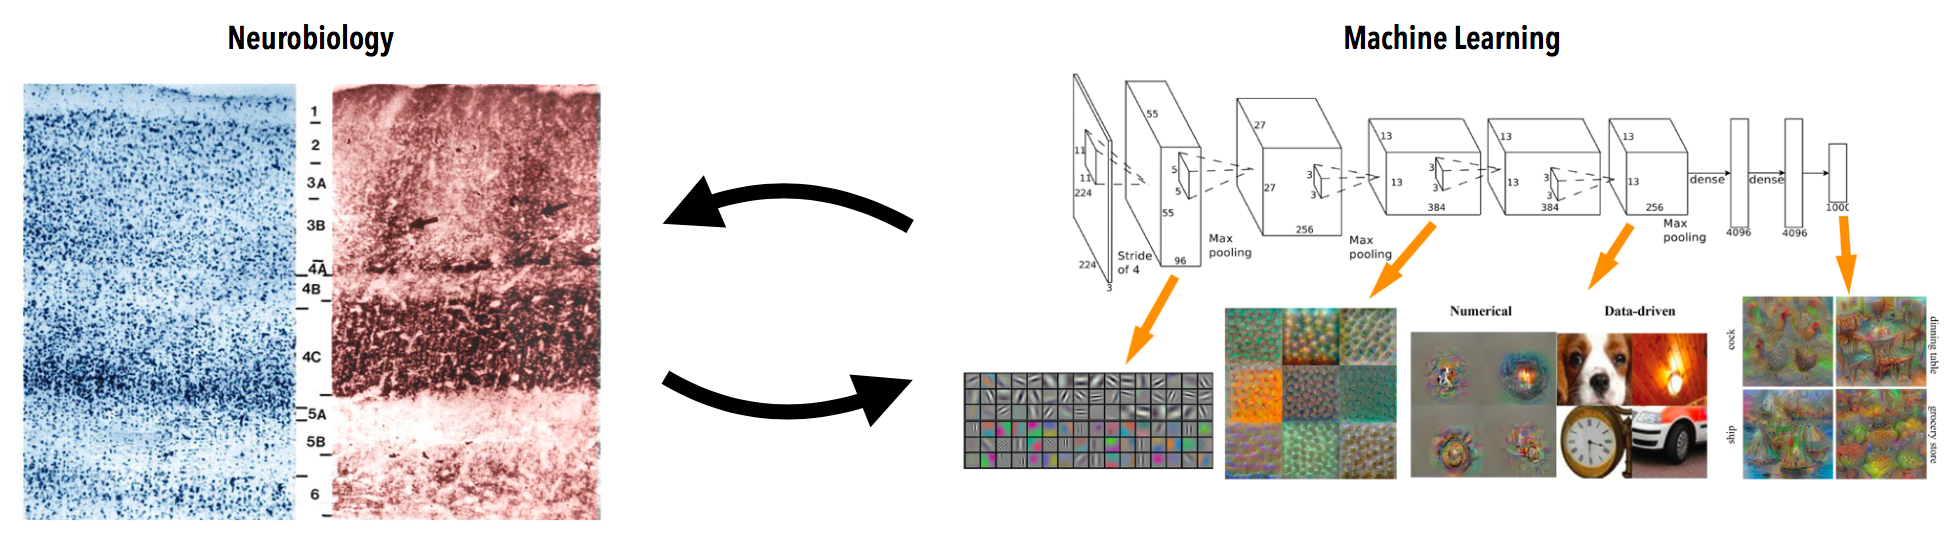
\includegraphics[width=\linewidth]{biology_vs_cnn.png}
%  \caption{The Biological Vision (schematic)}
%	\label{fig:vision}
%\end{figure}

Biological vision is an extremely powerful system which allows humans the ability, and seemingly without effort, to recognize an enormous amount of distinct objects in the world. 
Object detection is extremely difficult and therefore is especially impressive as light intensities can change by levels of magnitude and contrast between foreground and background is so often low. 
In addition, the visual scene changes every time the human body or human eyes move. 
This visual system exhibits a very noisy structure but because it is organized by layers it has inspired the mathematical theory of multilayer neural networks. 
What is remarkable is that even though current machine learning models do not resemble the complexity of its biological pendant, they inherently generalize extremely well. 
Neural networks trained on one specific task can be used to perform detection or segmentation of, seemingly, unrelated objects with relatively minor retraining. 
The reported classification performance is superior to that of humans and the question in regards to their functionality opens an interesting research topic.

In 1962 Hubel and Wiesel were the first to begin studying the visual cortex from the standpoint of a neuroscientist. Their experimental findings on cats and macaque monkeys suggested a hierarchy of cells with increasing complexity which was then later transferred to the hierarchical model of different layers. Twenty years later, this insight was translated to the Neocognitron quantitative model, by Fukushima and Miyake, which ultimately led to the important work of Hinton, Bengio, and LeCun in the 1980s. Their work on stochastic gradient descent approximation, and the availability of faster computer hardware then led to today’s breakthrough of deep learning networks. In the last decade, this field has exhibited rapid growth, constant evolution, and new applications in various domains.




GOALS
\begin{itemize}
	\item reduce the gap between neurobiology and data science to advance the understanding of visual cortex inspired machine learning
	\item insights for infovis for machines
\end{itemize}

CONTRIBUTIONS
\begin{itemize}
	\item experiments of cleveland mcgill with systematic parametrization and evaluation for computational perception
	\item ranking of elementary perceptual tasks for machine perception
	\item validation of weber's law for feedforward neural networks
	\item many insights for infovis for machines
\end{itemize}


